
% this file is called up by thesis.tex
% content in this file will be fed into the main document

%: ----------------------- introduction file header -----------------------
\begin{savequote}[50mm]
Historical methodology, as I see it, is a product of common sense applied to circumstances. 
\qauthor{Samuel E. Morison}
\end{savequote}


\newcommand{\codigo}[1]{``\texttt{#1}''}
\newcommand{\primquery}{\emph{query}}
\newcommand{\primread}{\emph{read}}
\newcommand{\primtake}{\emph{take}}
\newcommand{\primwrite}{\emph{write}}


\chapter{Triple Space Computing for resource constrained devices}
\label{cha:tsc}
\newcommand{\pathchapthree}{3_tsc}

% the code below specifies where the figures are stored
\ifpdf
    \graphicspath{{\pathchapthree/figures/PNG/}{\pathchapthree/figures/PDF/}{\pathchapthree/figures/}}
\else
    \graphicspath{{\pathchapthree/figures/EPS/}{\pathchapthree/figures/}}
\fi



% ----------------------------------------------------------------------




Although in the Chapter~\ref{} and Chapter~\ref{} we refine how they work.
Particularly, 
regarding its network layer.
To make \ac{tsc}'s shared space over the network an underlying network-based architectural style needs to be chosen.


In recent years, the \acf{iot} has became a reality due to the increasing number of everyday objects with computing and networking capabilities.
The use of these everyday objects together with the rising of mobile computing greatly contributes to the \ac{ubicomp} vision.
In the beginning the community put more effort on those devices' connectivity issues, materialized in the spread of technologies such as Zigbee\footnote{http://www.zigbee.org}, 6LoWPAN\footnote{http://datatracker.ietf.org/wg/6lowpan/charter/} or Bluetooth\footnote{http://www.bluetooth.com}.
However, nowadays it is focusing on the architectural solutions used by the applications built around these objects.
A model to classify this solutions has been already presented in the previous chapter. % Coulouris et al.


% defendemos usar TSC
In this thesis, we defend that \acf{tsc} provides some valuable properties to \ac{ubicomp} environments. % mencionarlas?
However, some other properties are derived from how \ac{tsc} is implemented.
In this chapter we focus on selecting the underlying network-based architectural style.
% TODO problema: y por qué no otros? Habría que redactarlo de tal forma que no haga que un lector tiquismiquis requiera un puto survey de network-based architectural styles!
%This style guides how \ac{tsc}'s shared space is accessed over the network.
% In the Chapter~\ref{} and Chapter~\ref{} we define...


The REST architectural style, defended by the \acf{wot} initiative, is probably the most prominent architectural solution used for smart-objects. % probably porque no tengo datos que lo defiendan
The benefits that REST brings to resource constrained devices have been deeply described in the previous chapter.
However, in Section~\ref{sec:rest} we analyze the characteristics of the style itself.

In Section~\ref{} we describe the similarities that \ac{tsc} has with the REST style.
Later, in Section~\ref{} we design a \ac{tsc} implementation which respects the REST principles.
The goal pursued is two-fold: (1) inherit most of the properties of REST and (2) maintain a high degree of compatibility with the \ac{wot}.
% on top of
% pros y contras



%    propiedades aportadas por REST a IoT

\section{On the \acs{rest}fulness of \acs{tsc}}
\label{sec:tsc_restfulness}

\subsection{\acl{tsc}}
\label{sec:tsc_vs_rest}

\ac{tsc} consist of a shared space which is accessed using some known primitives.
\emph{Per se}, \ac{tsc} does not contradict in any sense the \ac{rest} principles:

\begin{description}
 \item[\ac{restcs}.] Accessing to a space through a server in a \ac{restcs} fashion is completely feasible.
		      Indeed, this does not prevent to use a distributed solution in the \emph{back end} (e.g. a distributed semantic repository).
 \item[\ac{rests}.] The primitives to access the space imply simple read and writes which do not store any state in the server.
 \item[\ac{restcache}. ] The semantic content stored in the space can be cached.
                          However, the dynamism of the underlying network can make effective caching challenging to achieve. % quería poner "tune up" pero "configure" me ha sonado más fino
 %\item[\ac{rest_u}:] % lo quito porque si no, este punto sin texto con otros subpuntos queda feo
    %\begin{description}
	\item[\ac{restid}.] There are three types of identified resources in \ac{tsc}: spaces, \ac{rdf} Graphs and certain elements of the \ac{rdf} Triples.
	                 All of them are identified by URIs.
	                 The space can be seen as a coarse-grained view of the underlying graphs.
	                 The graphs have sets of triples which are usually related and describe a unit of knowledge. % A RDF triple by itself cannot transmit too much information
	                 Self-identified triple's subjects, predicates or objects are the source of concept linking.
	\item[\ac{restrep}.] The \ac{rdf} graphs and triples mentioned above can be represented using different standard serializations.
			      %Nevertheless, 
			      % citar el paper que habla de cómo alinear LOD y REST
	\item[\ac{restdesc}.] The messages derived from the primitives are self-describing since they are expressed on standard \ac{rdf}-based languages. % including meta-data
				Therefore the server and clients know how to process the content according to its language and certain vocabularies.
				These vocabularies specifications (i.e. ontologies) are referenced in the content.
	\item[\ac{resthateoas}.] The lack of native hypermedia support in \ac{rdf}-based representations make this the most challenging property to achieve \citep{page_rest_2011}. % compara LOD y REST
				  However, some recent works propose means to fulfill this property.
				  \citet{kjernsmo_necessity_2012} proposes a vocabulary for hypermedia \ac{rdf}.
				  \citet{steiner_fulfilling_2011} and \citet{verborgh_functional_2012} propose to enrigh the \ac{http} header with hypermedia information.
				  While the first changes representations, the latter is a more general way to provide hypermedia.
    %\end{description}
 \item[\ac{restl}.] Encapsulation of functionalities can be achieved through a layered system.
                     For example, to balance the load to a space replicated in two machines.
 % TODO TODO repensar si ontologías, reglas y demás (personalizar behavior) se puede entender cómo COD:
 % In the code-on-demand style [50], a client component has access to a set of resources, but
 %  not the know-how on how to process them. It sends a request to a remote server for the
 %  code representing that know-how, receives that code, and executes it locally.
 \item[\ac{restcod}.] Although it may not be as common as scripting in ordinary human-browsing, % TODO reexplicar esto mejor?
            the \emph{know how} can be downloaded from the server in several ways:
            \begin{enumerate}
	      \item Modeling scripts using appropriate ontologies. % TODO cite
	      \item A semantic reasoner can be considered an interpreter for the content downloaded from the server.
	            It is used to extract unstated information from the content received from the server.
	            Therefore, the client downloads know-how to process the resource in the following situations:
		    \begin{itemize}
		      \item Through the taxonomies defined in ontology files. % e.g. para hacer un mapeo; en analogía a JS, da igual que tu tengas previamente el script o no
		            This taxonomies are modeled using standard semantic languages. % hablar de distintos niveles de expresividad?
		      \item Through semantically expressed rules \citep{berners-lee_n3logic:_2008}. % (e.g. N3 rules)
		    \end{itemize}
	      % con nuevo TBox que te bajas??
            \end{enumerate}
\end{description}



\subsection{Aligning \acs{tsc} with \acs{http}}
\label{sec:align_tsc_http}

% TODO Revisar cosas del texto original que no encajaban aquí (están comentadas)
% TODO citar trabajos de:
%      TSC es como Web para semántica
%      RESTful semántico
%      So far, the compatibility of \ac{tsc} with the \acs{http} RESTful style has been proved from a formal \cite{hernandez_formal_2010} point of view.
%      Papers sobre TSC y su discurso sobre la WWW

In this section, we present a \ac{tsc} \acs{api} over \ac{http} to give a practical overview of \ac{tsc}'s \acs{rest}fulness.

\subsubsection{\acs{tsc} resources}

Three key concepts are important to understand the resources in our proposal: agents share information in a common \textbf{space}.
A space is identified by an \acs{uri}.
Therefore, all the operations in \ac{tsc} are performed against a particular space.
%By default, all applications connect to a common standard space, but they can optionally choose to connect to a particular private space.
Within a space, the information is stored in sets of \textbf{triples} called \textbf{graphs}.
Each graph can also be identified by an \acs{uri}.
The \acs{rdf} \textbf{triples} are the underlying concept of all the \ac{sw} languages.
Each triple is composed by a subject (which is a \acs{uri} or a \emph{blank node}), a predicate (a \acs{uri}) and a value (which can be a \acs{uri}, a \emph{blank node} or a literal), as shown in the Figure~\ref{fig:triples_example}.
% TODO cuidado con los blank nodes!!! Los tenemos en cuenta? De ser así, cómo???

As detailed later, \ac{tsc}'s primitives add or remove graphs.
% este es un tema "delicado" desde el punto de vista de TSC, así que mejor si lo tratamos a parte:
% as well as to query for graphs or for sets of triples retrieved from different graphs.
In order to perform these operations, which enable the selection of a subset of the semantic content hold in a given space, a \textbf{template} is required. % these operations: add or remove
The wildcard templates used by default
\footnote{
  % Por qué no SPARQL?
  More sophisticated query languages like SPARQL (\url{http://www.w3.org/TR/rdf-sparql-query/}) could be used. % sophisticated o expressive?
  However, not many embedded platforms have parsers for these languages available.
  This could be an obstacle for the adoption of the middleware.
  Therefore, we have opted for using wildcard templates, which are in turn much more simple to process.
  In any case, the nodes able to parse these query languages can easily decompose a query on wildcard templates.
}
are special triples with optional wildcard subject, predicate and/or object.
For example, the template \texttt{?s foaf:knows gomezgoiri:aitor} could be employed to select instances which represent people who know Aitor (see Figure~\ref{fig:tsc_resources}).

% TODO Discussión profunda de SPARQL y REST???

\InsertFig{tsc_resources}{fig:tsc_resources}{
  Schematic view of a space with four graphs and sample triples for one of these graphs.
}{
  Aliases for the beginning of most URIs, known as prefixes in most Semantic languages, are used for the lack of clarity.
}{1}{}


\subsubsection{Adopted \acs{tsc} primitives}
\label{sec:primitives}

\acs{tsc} derives some primitives originally defined in the Linda language \citep{gelernter_generative_1985} to access to the semantic information hold in each graph.
In this section, we explain these primitives.

\begin{itemize}
 \item The \textbf{write} primitive allows writing a graph into a given space (identified by its \acs{uri}).
	The set of triples received by this primitive will be stored together in the same graph, returning the \acs{uri} which identifies that graph.
	The graph \acs{uri} can be used to access directly to that graph later on, or to create new triples and relate contents.
       % Esto no encaja necesariamente con el concepto de "Browsable graph": http://www.w3.org/DesignIssues/LinkedData
  \begin{lstlisting}
    write(space_URI, triples): URI              [1]
  \end{lstlisting}


  \item The \textbf{read} returns a graph belonging to a given space which contains at least a triple matching the given template or has the given \acs{uri} as its identifier.
	If more than one graph fulfill one of these conditions, just one of them is returned (nondeterministically).
	It should be remarked that it has been designed as a non blocking operation.
  \begin{lstlisting}
    read(space_URI, graph_URI): triples         [2]
    read(space_URI, template): triples          [3]
  \end{lstlisting}
  
  
% why?
% TODO READ al ser no-deterministica puede afectar a caching???
  \item The \textbf{take} primitive behaves like a destructive \textbf{read}, deleting the graph returned from the space.
  \begin{lstlisting}
    take(space_URI, graph_URI): triples         [4]
    take(space_URI, template): triples          [5]
  \end{lstlisting}

%  \item Space management primitives.
%	A node can join or leave a space using \linebreak \texttt{joinSpace(space\_URI)} or \texttt{leaveSpace(space\_URI)}.
\end{itemize}



\subsubsection{\acs{http} \acs{api} for \acs{tsc}}
\label{sec:httpapi}

As both \ac{tsc} and \ac{http} are \ac{rest} compliant, their similarities are evident.
In the same way \ac{tsc} has the already explained primitives, \ac{http} has verbs to get, create, update or remove resources (GET, PUT, POST, DELETE).
%The main purpose of \acs{tsc} primitives is not to access data but to coordinate the nodes accessing to that data.
Consequently, the translation between these two worlds is straightforward.

\begin{sloppypar}
According to the \ac{rest} principles the interaction with an API must be hypertext-driven \citep{fielding_rest_2008}.
To ease its usage by developers, we provide a human-oriented \acs{html} representation of the \ac{api} which is completely \emph{browseable}.
% un poco repetido de la parte de HATEOAS
Regarding the machine-oriented (i.e. semantic) representation of the \ac{api}, several solutions to enable hypermedia driving have been proposed by \citet{verborgh_functional_2012} and \citet{kjernsmo_necessity_2012}. % mencionar que son experimentales?
Independently of the mechanism adopted, in this section we propose a optional \ac{api} which tries to stress \ac{tsc}'s compliance with \ac{http}.
\end{sloppypar}

The list of spaces a node is joined to are available under \textit{/spaces}.
Each space is identified by an \acs{uri} (e.g. \url{http://space1}).
All the resources of that space, both real (i.e. graphs) or virtual (i.e. query) are listed under $/spaces/\{space\_uri\}$ (summarized by \emph{sp} from now on).
Each graph is available on ${\{sp\}/graph/\{graph\_uri\}}$.
If we make an \acs{http} DELETE to that resource, under \ac{tsc}'s perspective, we take that graph from the space.
The rest of the mappings are shown in the Table~\ref{tab:tscAPI}.

\begin{table} %http://en.wikibooks.org/wiki/LaTeX/Floats,_Figures_and_Captions#Wide_figures_in_two_column_documents
  \centering
  \caption {
    \acs{http} mapping for the primitives detailed in the Section~\ref{sec:primitives}. \textit{sp} is a space \acs{uri},
    \textit{g} is a graph \acs{uri}, \textit{s}, \textit{p} and \textit{o-uri} are subject, predicate and object \acsp{uri} or wildcards (represented with an as \textit{*}).
    When the template's object is a literal, it can be expressed specifying its value (\textit{o-val}) and its type (\textit{o-type}).
    \medskip
  }
  \begin{tabular}{c|l|c}
      \acs{http} request & \acs{url} & Returns \\
      \hline
      POST & \{sp\}/graphs/ & [1] \\
      GET & \{sp\}/graphs/\{g\} & [2] \\
      GET & \{sp\}/graphs/wildcards/\{s\}/\{p\}/\{o-uri\} & [3] \\
      & \{sp\}/graphs/wildcards/\{s\}/\{p\}/\{o-type\}/\{o-val\} & \\
      DELETE & \{sp\}/graphs/\{g\} & [4] \\
      DELETE & \{sp\}/graphs/wildcards/\{s\}/\{p\}/\{o-uri\} & [5] \\
      & \{sp\}/graphs/wildcards/\{s\}/\{p\}/\{o-type\}/\{o-val\} & \\
  \end{tabular}
  \label{tab:tscAPI}
\end{table}


\paragraph{Status Codes}
\label{sec:status_codes}
The \acs{api} should be compliant with the standardized \acs{http} status codes.
These codes are sent back in the response as part of the header.
For instance, the \ac{tsc} middleware returns the 404 error when no significant result can be found for a primitive.
This adoption, apart from enhancing the compatibility with other web applications, could enable the modular adoption of the API.
For example, if a node does not offer a wildcard based \textit{query}, it will not affect the behavior of the rest of the nodes of an space.
Instead, they will interpret these cases as empty responses.
This modularity becomes crucial to ease the partial adoption on new platforms.

\paragraph{Content Negotiation}
Another key aspect of the \acs{http} protocol the \acs{api} should take advantage of is the \textit{content negotiation}.
This mechanism allows to specify the desired representation for a content on the client side and to express what representation is sent as a response from the data provider side.
For that purpose, the client adds an \textit{Accept} field to the \acs{http} header with a weighted list of media types it understands.
Then, the server will answer with the best possible format it knows about, specifying the \textit{Content-type} in the response.

The benefits of using this mechanism in the \ac{tsc} middleware presented are two-fold.
Firstly, it enhances the browsability of the primitives with human understandable \acs{http} responses. % no sé si esto es de Content Negotiation per se
Secondly, it allows different semantic representations (e.g. RDF/XML\footnote{\url{http://www.w3.org/TR/REC-rdf-syntax/}}, N-Triples\footnote{\url{http://www.w3.org/2001/sw/RDFCore/ntriples/}} or N3\footnote{\url{http://www.w3.org/TeamSubmission/n3/}}).
The latter characteristic becomes crucial since not all the nodes may understand all the formats (e.g. a mobile phone may not have a RDF/XML parser).
%This is true even if all the languages use the same basic concepts (i.e. \acs{rdf} Triples).
In these cases, the compatibility of both sides can be ensured through a conversion carried out in the server side.
Furthermore, expressing the preference for a semantic format can be useful too in other cases.
For example, to obtain the less verbose answer.

\section{Distributed \ac{tsc}}
\label{sec:distributed_tsc}

% cómo y porqué hacer un TSC distribuído
In Section~\ref{sec:tsc_vs_rest} section we showed how \ac{tsc} can comply with all the constraints of the \ac{rest} style.
One of these constraints is that the access to a space is done in client-server basis.
The easiest way to achieve this constraint is by centralizing all the content of each space in the server itself.


% Pero un entorno Ubicomp es eminentemente distribuído
However, the data in a \ac{ubicomp} environment is not generated in a single point.
%   La información se genera en fuentes separadas, ¿cómo accedo a los últimos datos?
In fact, each sensor in an intelligent environment is potentially generating data constantly.
Besides, the magnitude of this sensors can be enormous.
This creates a trade off between efficiency and update difficult to overcome:
\begin{itemize}
  \item The more frequently each sensor sends contents to the server, the more inefficient is the solution in terms of network usage.
  \item The less frequent this communication is, the less updated is the data in the server.
        This leads to spaces which misrepresent the environments.
\end{itemize}
A sensitive solution is to let these sensor manage their own information.


%   ademas no practico:
%        las fuentes del conocimiento son las que mejor saben como gestionar una informacion (crearla, acualizarla o eliminarla)
%        la información se transporta en dispositivos
%        reusar datos en distintas apps
Furthermore, this strategy can not only be useful for devices which constantly generate new data.
Delegating responsibilities between the devices presents additional benefits:
\begin{itemize}
  \item They will know how to represent these contents better than others. % ejemplo en grados centigrados o celsius?
	For example, the unit of a temperature measure.
  \item They know when to create, update or delete data. % ejemplo if a server receives 2 contradictory measures... algo
        In fact, they can opt for creating data on demand.
  % TODO esto es más un beneficio de REST que de otra cosa
  \item The data can be reused by other applications or even other spaces. % Interop!
        These applications would not be required to use a space-based approach.
        Therefore, they will not depend on the correct functioning of our whole system. % del servidor central
  \item Carrying that information can be useful in certain mobility situations.
        For example, let a us imagine a person which stores her user profile in the smartphone.
        She could share it with different spaces or applications as it moves along the city.
\end{itemize}


% Aún así, que los dispositivos se coordinen a través de una entidad central es conveniente:
%       Sencillo de implementar: notificaciones, razonamiento, etc.
%       Incluso si ese espacio luego está distribuído o cambia de máquina, acceso a través de dicha interfaz (HTTP o CoAP el día de mañana)
%       Modo: caching (para reliability) o modo ver qué hay en el espacio ahora mismo (visión en tiempo real)
%       -->> INDEPENDENCIA DE LOCALIZACIÓN!!!
Still, most of the \ac{iot} devices or mobile phones are unreliable: they can join and leave at any moment.
Therefore, distributing the shared space among unreliable nodes comes with a number of drawbacks:
\begin{itemize}
  \item This unreliability makes difficult to maintain the consistency of the space. % TODO CUIDADO, puedo estar metiendome en un fregado, la parte de los dispositivos no será consistente!
        Since this information drives the coordination between the devices, its consistency is important.
  \item A blocking mechanism is important in space-based computing.
        For example, a worker node may block until some task is become available in the space.
        A way to implement it in a distributed space is by means of a notification system.
        Again, implementing it using unreliable devices is hard to implement. % no sé si esto último no sonará demasiado a mofa...
  \item And last but not least, if the access to some data in the space cannot be guaranteed no matter if the device which wrote that information is available, there will not be \emph{time uncoupling}.
\end{itemize}
Overcoming the previous difficulties, usually implies a high network traffic.
However, this negatively influences the energy consumption of nodes whose energetic autonomy might be limited.


\subsection{A Halfway Solution}
\label{sec:halfway_solution}

In this thesis, we propose to conserve the desirable characteristics of both \ac{rest} and \ac{tsc} by mixing them.

On the one hand, we propose a uniform access to the space by the \acs{http} \ac{api} described previously.
The space can then be distributed using any existing approaches. % TODO cite
However, for the sake of clarity, we will assume that each space is managed by a unique server.

On the other hand, each space will be enriched by the data provided by various autonomous providers.
These providers might be any kind of mobile or embedded device, no matter how limited they are.
This \emph{enrichment} can be materialized:
\begin{enumerate}[(a)]
  \item Considering additional data in a reasoning process triggered when a primitive is called.
  \item Including additional data as a response.
        For example, a graph read from an embedded device could be returned as a response to a primitive.
\end{enumerate}
In this thesis, we have focused on the latter alternative.


To do that, we propose an extension of the already presented \ac{tsc} model by means of new concepts, new primitives and new behavior.
Figure~\ref{fig:new_model} presents the key elements of this new model.


\InsertFig{new_model}{fig:new_model}{
  Key concepts of the new \ac{tsc} model presented.
}{
  The coordination space, is where the graphs can be written, read and taken by any participant.
  The coordination space is hold by a device called \emph{coordinator}.
  The current view of all the \emph{self-managed graphs} in the space forms the \emph{outer space}.
  Therefore, the \emph{outer space} is hold by many devices (also called \emph{asteroids}).
  The \ac{tsc} \ac{http} \ac{api} corresponds with the generic \ac{tsc} to access to the primitives presented in Section~\ref{sec:align_tsc_http}.
  The \emph{OSAPI} is the \ac{api} which must be implemented by any node willing to share \emph{self-managed graphs}.
}{1}{}


% grafos autogestionados (no takeables por otros) => write en local
\subsubsection{Self-managed graphs}

These graphs are the ones which are managed by the device, called \emph{asteroid}, which provides them to the rest.
In other words, self-managed graphs enrich the space in the ways previously described, but they cannot be removed.
% poner ejemplo de por qué no tiene sentido que eliminen a través del espacio
Therefore, they are \emph{second-class graphs} which provide information about the environment but cannot be used for coordination purposes.

% write locally
% No device can remove them apart from their creator. % TODO o si puede serlo, esta no lo decide el sistema
The \emph{asteroid} makes these graphs accessible to others through \ac{http}.
% objetivo: que se pueda acceder a estos grafos incluso si no son parte de nuestra app => interop
The final goal is to potentially allow to reuse the data provided by any existing \ac{rest}ful service. % app level interop
Therefore, the \ac{api} should be or trend to be \ac{rest}ful.
% para ello es importante usar un RESTful approach, como sabemos que es complejo ofrecemos otra opción en el siguiente capítulo
However, we leave the \emph{hypermedia} \ac{api} as a future work.
Instead, we require a mandatory \emph{OSAPI} to be implemented in each \emph{asteroid} to guarantee access to the \emph{self-managed graphs}.
% lo sé, no está justificado 0:-)



\subsubsection{New primitives}

To make the most of the information in a space, we propose a new primitive to query all over the semantic information stored.
The \ac{rest}fulness of this primitive could be argued since it does not operate at resource level, but mixing several resources.
However, we believe that it is useful to have an endpoint for the queries which involve many graphs.
\citet{kjernsmo_necessity_2012} discusses this topic in depth. % TODO Mirar otras citas???

This new primitive is defined as follows:
\begin{itemize}
  \item The \textbf{query} primitive aims to see the space as a whole, returning all the triples matching the given template.
  
  \begin{lstlisting}
    query(space_URI,template): triples          [6]
  \end{lstlisting}
\end{itemize}


The Table~\ref{tab:queryAPI} extends Table~\ref{tab:tscAPI} to include this new primitive.
% TODO otra clave: debería no tener porqué pasar por el servidor

\begin{table} %http://en.wikibooks.org/wiki/LaTeX/Floats,_Figures_and_Captions#Wide_figures_in_two_column_documents
  \centering
  \caption {
    \acs{http} mapping for the primitives detailed in the Section~\ref{sec:primitives}. \textit{sp} is a space \acs{uri},
    \textit{g} is a graph \acs{uri}, \textit{s}, \textit{p} and \textit{o-uri} are subject, predicate and object \acsp{uri} or wildcards (represented with an as \textit{*}).
    When the template's object is a literal, it can be expressed specifying its value (\textit{o-val}) and its type (\textit{o-type}).
    \medskip
  }
  \begin{tabular}{c|l|c}
      \acs{http} request & \acs{url} & Returns \\
      \hline
      GET & \{sp\}/query/wildcards/\{s\}/\{p\}/\{o-uri\} &  [6] \\
      & \{sp\}/query/wildcards/\{s\}/\{p\}/\{o-type\}/\{o-val\} & \\
  \end{tabular}
  \label{tab:queryAPI}
\end{table}


A key point of the \ac{api} is that the \emph{asteroids} might not even follow the \ac{tsc} paradigm.
For instance, the \emph{OSAPI} can encapsulate data provided by a third middleware.
However, a primitive to ease that management can be a convenient for the developers which do not need a more customized behavior.
With that in mind, we propose another writing primitive.
This primitive only has local effects and therefore has no HTTP equivalent:
\begin{itemize}
  \item The \textbf{write\_self} primitive writes a \emph{self-managed graph} and returns an \ac{uri} which identifies it.
  
  % tiene sentido definir el space_URI???
  % mejor definir su propio espacio?
  % tiene sentido especificar su URI? write_self(graph_URI, triples): URI
  \begin{lstlisting}
    write_self(space_URI, triples): URI
  \end{lstlisting}
\end{itemize}



\subsubsection{New behaviors}

% explicar cómo se escribe y lee en el espacio
% solución enfoque híbrido:
%      cambios en actuadores => directamente a través de HTTP o indirectamente a través de tasks escritas en espacio
%                               o mejor: podrían esas tasks ser directamente esos servicios???
%      grafos que sí => write al "servidor HTTP"
%      query => en todos los dispositivos (capítulo 4) - Porque a veces es necesario a través de todos los nodos
%      take + read => sobre los grafos takeables (o inferencia con toda la info del espacio, cómo prefieras)
In this section we will try to clarify how the different behaviors coexist.

\paragraph{Writing}

The most basic writing primitive allows a client to write a graph into the space hold by the server.
However, we also presented the \emph{write\_self} primitive.
\emph{Write\_self} writes into the local device a untakeable graph (i.e. self-managed graph).
% TODO comprobar una vez acabado que es así!
Finally, in Chapter~\ref{cha:actuate} we argue that a third \emph{writing} primitive is necessary.
This primitive should allow to \emph{suggest} physical changes in the space through actuators.


\paragraph{Reading}

\emph{Query} performs a traversal query which aggregates all the graphs of the space.
\emph{read} and \emph{take} work at resource level.
However, we will also consider \emph{self-managed graphs} to enrich the \emph{read} primitive. % mediante redirect o lo que sea
\section{Conclusions} % TODO llamarlo Evaluation?

With the solution presented in the previous section, we aimed to retain the desirable properties of both \ac{rest} and \ac{tsc}.
% analísis más largo en la siguiente sección
% 1. cómo sé que esto es mejor que usar REST y TSC por separado? Sinergia?
% 2. que aporta unirlo bajo un mismo middleware?
% 3. tiene beneficios?
However, some questions arise from that integration:
(1) does in fact retain all the properties of \ac{rest} and \ac{tsc} separately? Otherwise, which properties are affected?
(2) what other benefits carries comparing with using already existing \ac{tsc} and \ac{rest} middleware?

% Fielding distingue entre:
%      + "distributed-system": hace que el usuario vea el sistema como un todo, sin saber cuando se realizan llamadas en remoto y cuando no
%      + "networking-system": no necesariamente oculta las particularidades de la red <- el se centra en estos


To answer these questions, we analyze the presented solution from different point-of-views:
(1) its coordination properties (Section~\ref{sec:XXX_properties}),
(2) its network-level properties (Section~\ref{sec:network_properties}),
(3) how the latter work together to contribute to the challenges of an \ac{ubicomp} environment (Section~\ref{sec:middleware_properties}).
Section~\ref{sec:middleware_eval_summary} summarizes these analysis. % cómo dan respuesta a las preguntas del comienzo


% TODO cosas rescatables del paper original de WoT 2011:
%     Uniform API vs. specific usage of each API !!!
%     Coupling: lo comido (autonomies), por lo servidor (client-server coupling por tener API común)
%          In spite of the outlined decoupling nature of both approaches, the data definition can be considered a coupling mode indeed.
%          While in \ac{wot} each resource defines its own data formats and contents themselves, in \ac{tsc} the ontology in which the semantic
%          concepts are described must be known by each part of a distributed application to effectively cooperate among them.
%     Discovery: HATEOAS puede ser complejo para cacharros peques (parseo),
%                proponemos discovery basada en API uniforme y a nivel de cacharros con algún mecanismo en el que no entramos.
%          One of the main drawbacks in \ac{wot} is the lack of a discovery mechanism for new objects and the data they provide.
%          Even when this data can be linked in each object response (using HATEOAS) and microformats are sometimes included to ease the search-ability of these objects by search engines, it is difficult for an object which may change of location and context to be referred.
%          Thus, \ac{wot} may have a tendency to create isolated islands of data.
%          Several workarounds have been proposed to overcome this limitation, such as using a central repository\footnote{http://www.pachube.com/}, a framework which uses federated repositories responsible for different administrative domains \citep{stirbu_towards_2008} or making each connected sensor announce itself to let an intermediary know its presence \citep{kamilaris_smart_2010}.

%     Scalability: se ha hablado y ahora no es tan mala como antes ;-) Entre cacharros seguiría dando asco
%     Semantics: Microformats vs Full (hablar de esto)
%     Comprensión por parte de usuario: sencillo misma interfaz, no tienes que andar descubriendo nuevas APIs y viendo cómo funcionan, qué formato devuelven, etc.
%     Comprensión por parte de desarrollador: API sencillica siempre


\subsection{Coordination properties}
\label{sec:coordination_properties}

% TODO añadir la autonomía que se refería a la semántica?
As we have already discussed in Section~\ref{sec:integration}, indirect communication middleware can have two key properties:
\begin{itemize}
  \item The sender does not need to know the receiver or receivers and vice versa (i.e. \emph{space uncoupling}).
  \item Senders and receivers do not need to exists in the same time to communicate with each other (i.e. \emph{time uncoupling}).
\end{itemize}


The primitives used in our space-based computing implementation force it to be \emph{space uncoupled}.
On the contrary, it is not always \emph{time uncoupled}.
If two nodes write and read from the coordination space, they are \emph{time uncoupled};
but if a node accesses to others' content (i.e. \emph{self-managed graphs}), they are not.
In other words, \emph{time uncoupling} is not achieved by the extension of the model presented in Section~\ref{sec:halfway_solution}.
As a future work, this could be alleviated by a caching mechanism implemented in the space holder or holders. % TODO hablar con propiedad de esos elementos => nombrarlos antes
% see \ref{tab:middleware_coordinationprop}


% Tablita de cómo hereda propiedades de los estilos anteriores?
% (y si quieren más información, que miren en la tesis de Fielding)
\begin{savenotes} % to use footnotes inside
  \begin{table}[htbp]
    \caption{Uncoupling levels achieved by the different parts of the middleware presented.}
    \begin{center}
      \begin{tabular}{lcc}
	\hline
	~ & Space &	Time \\
	~ & uncoupling & uncoupling \\
	\hline
	% O mejor ponerlo con Yes y No?
	Coordination space & $\checkmark$ & $\checkmark$ \\
	Outer space & $\checkmark$ & × \\
	\hline
      \end{tabular}
    \end{center}
    \label{tab:middleware_coordinationprop}
  \end{table}
\end{savenotes}


\subsection{Networking properties} % Architectural Properties for Network-based Styles
\label{sec:network_properties}
% Cómo afecta la app propuesta => ir actualizando al final de otras secciones???

In Section~\ref{sec:tsc_vs_rest} we have described how \ac{tsc} does not contradict any of the \ac{rest} principles.
However, the adaptation presented in this thesis does not completely adhere to the \ac{rest} style.
In this section we present how this divergences affect the \ac{rest}'s properties.
% decir que el objetivo final es que pudiera ser REST

% TODO antes de entrar al lio, explicar cómo funciona esto de REST, en qué parte de nuestra solución lo necesitaremos
% decir que API para TSC mola
% decir que API para los cacharros deberia de ser independiente a lo que nosotros digamos y por eso estaria bien REST
%     de todas formas, como es dificil, nos quedamos en un nivel de madurez menor


In \citeauthor{fielding_architectural_2000}'s words, the relevant properties which describe a network-based system are the following ones \footnote{We refer to the reader to \citet{fielding_architectural_2000} for the complete thorough analysis.}:
% verificar que no se parece demasiado a sus definiciones o sino poner cursiva.
\begin{description}
  \item[Performance] is divided into network performance, user-perceived performance and efficiency.
    \begin{description}
      \item[Network performance] is affected by the styles in the number of interactions and the granularity of data elements.
      \item[User-perceived performance] refers to the impact a user in front of an application perceives. % UP Performance es una feature que no aporta mucho a nuestro caso
      \item[Efficiency] is achieved by minimizing the use of the network.
    \end{description}
  \item[Scalability] measures how an architecture supports a big amount of components and interactions between them.
  \item[Simplicity] is achieved through the separation of concerns for the components and the generality of architectural elements.
  \item[Modifiability] encompasses evolvability, extensibility, customization, configurability and reusability.
    \begin{description}
      \item[Evolvability] refers to the degree in which a component can be implemented without negatively impacting on others.
      \item[Extensibility] measures the ability to add functionality to the system.
      \item[Customization] is the ability to customize the behavior of an architectural element temporarily.
      \item[Configurability] is related with the extensibility and the reusability.
      \item[Reusability] is the ability to reuse components, connectors or data elements without modifying other apps.
    \end{description}
  \item[Visibility] is the ability of a component of monitoring or mediating in the interaction between other two components.
  \item[Portability] is the ability of working in different environments.
  \item[Reliability] is the degree in which an architecture depends on the failures of the system or components, connectors or partially incorrect data.
\end{description}

% Requisitos de ealy web, propiedades deseables
%   Low entry-barrier
%   Extensibilidad
%   Distributed Hypermedia
%   Internet-scale

The Table~\ref{tab:network_properties} summarizes how different architectural styles achieve these properties.
Particularly, it shows the styles from which \ac{rest} derives (see Section~\ref{sec:rest}).
The ultimate goal of the solution explained in the previous section is twofold:
\begin{enumerate}
  \item Provide a \ac{rest} access to a semantic space.
       This would ease its integration with the rest of the web.
  \item Enrich that space with the knowledge provided by other \ac{rest} \acp{api}.
\end{enumerate}
Therefore, ideally, its networking properties would be the sames as the \ac{rest} style.


However, defining a 100\% \ac{rest} compliant \ac{api} is not easy.
Indeed, most of the self-proclaimed \ac{rest}ful \acp{api} are not \citep{house_how_2012}. % la nueva buzz word para eso: hypermedia API
The main cause is the \emph{HATEOAS} constraint seen in the Section~\ref{sec:rest} \citep{fielding_rest_2008}.
Using \ac{http} as an application-level protocol forces a developer to comply the rest of the constraints \citet{moore_hypermedia_2010}, but not \emph{HATEOAS}.
% TODO hablar del Richardson Maturity model!


% semantic-based \ac{api} is not easy. => referencias a los que lo han intentado, a que no hay hipertexto, a que te puede interesar inferir con bastantes
Regarding the \ac{sw}, some recent efforts have tried to move closer to the \ac{hypermedia} constraint \citep{steiner_fulfilling_2011,kjernsmo_necessity_2012}.
However, these worlds remain quite isolated.
In fact, \ac{sw} API  usually present another main divergence with the \ac{rest} style: the use of query endpoints.
% i.e. no devuelven listas de enlaces, sino todo a lo bruto
% esto quiere decir que no se devuelve todo y ala, tu procesa esa burrada de datos, más bien se filtran
These endpoints intend to solve some inefficiency issues which \ac{rest} shows when working with a big amount of data. % TODO mencionar \ac{lod} en algún punto de aquí?
To that end, they allow expressive query languages and offer results where the boundaries of the different resources often blurs \citep{wilde_restful_2009}.
The most paradigmatic case may be to decide to which graph does a inferred content belongs. % ejemplo de lo anterior


% Aterrizar esto a IoT y a nuestro caso:
%        La eficiencia es importante => para evitar hacer 500 llamadas a un cliente
%        La reusabilidad es importante también => para potencialmente adaptarse a cualquier WoT semántico
%           en el futúro => más trabajo en este área
%       Solución de compromiso:
%           nivel de madurez X de Richardson. Suponemos que alguien debe serguir nuestro API mínimo en los objetos WoT

In \ac{iot} both the efficiency on the communications and reusability of the \ac{api} are important:
\begin{description}
  \item[Efficiency:] mobile and embedded devices' have restricted energy autonomy.
                    This autonomy is severely affected by network communications. % TODO cite
                    Particularly, the access to the data they provide by means of hyperlinks may result in many HTTP requests. % aunque eso se puede adaptar por lo visto
                    %  Por que sería muy costoso hacer rollo araña?!
		    %     lo que ganas de reusabilidad, lo aumentas en complejidad en el cliente
                    %     interpretar código del servidor no es tampoco super-sencillo (xHTML!)
  \item[Reusability:] due to the heterogeneity of the devices, assuming that they all share a common and unevolvable \ac{api} may not be realistic. % TODO paliar para que no parezca que no tiene sentido
\end{description}
The first solution together with the current difficulties on achieving a fully and standard \emph{HATEOAS} for machines in the \ac{sw}, lead us to opt for the second level on the Richardson Maturity level.
Besides, our \ac{tsc} \ac{api} will be \emph{HATEOAS} \ac{api} in its humans representation to ease their learning level.% pero aún así el API de TSC seguirá siendo HATEOAS para los usuarios, no para las máquinas
However, we do not discard to work towards a fully \ac{rest}ful \ac{api} as future work.


In conclusion, the properties of the properties for network communication style we adopted corresponds with \emph{LCODC\$SS} plus simplicity and visibility. % hacer una nueva fila con esto
% TODO comprobar que se explica eso tal cual en la tesis de Fielding: HATEOAS => sólo afecta a reusabilidad

% TODO Comprobar que no se salga por el borde derecho!

% Tablita de cómo hereda propiedades de los estilos anteriores?
% (y si quieren más información, que miren en la tesis de Fielding)
\begin{savenotes} % to use footnotes inside
  \begin{table}[htbp]
    \caption[Properties of different architectural styles for network-based applications as defined by \citet{fielding_architectural_2000}.]
            { Note that apart from including \ac{tsc}, the original table has been slightly adapted.
              These adaptations are defined inside the table. % using several footnotes.
            }
    \begin{center}
      \begin{tabular}{lccccccccccccc}
	Style &
	\rotatebox{90}{Net Perform} &
	\rotatebox{90}{UP Perform} &
	\rotatebox{90}{Efficiency} &
	\rotatebox{90}{Scalability} &
	\rotatebox{90}{Simplicity} &
	\rotatebox{90}{Evolvability} &
	\rotatebox{90}{Extensibility} &
	\rotatebox{90}{Customiz.} &
	\rotatebox{90}{Configur.} &
	\rotatebox{90}{Reusability} &
	\rotatebox{90}{Visibility} &
	\rotatebox{90}{Portability} &
	\rotatebox{90}{Reliability} \\
	\hline
	CS & ~ & ~ & ~ & $+$ & $+$ & $+$ & ~ & ~ & ~ & ~ & ~ & ~ & ~ \\
	S\footnote{\emph{S} represents the difference between \emph{CSS} and \emph{CS} in \citep{fielding_architectural_2000}.}
	  & $-$ & ~ & ~ & $+$ & ~ & ~ & ~ & ~ & ~ & ~ & $+$ & ~ & $+$ \\ % = CSS - CS
	\$ & ~ & $+$ & $+$ & $+$ & $+$ & ~ & ~ & ~ & ~ & ~ & ~ & ~ & ~ \\
	\hline
	Early web\footnote{Corresponds to the \emph{C\$SS} style in \citep{fielding_architectural_2000}.}
	 & $-$ & $+$ & $+$ & $++$ & $+$ & $+$ & ~ & ~ & ~ & ~ & $+$ & ~ & $+$ \\ % = C$SS
	L & ~ & $-$ & ~ & $+$ & ~ & $+$ & ~ & ~ & ~ & $+$ & ~ & $+$ & ~ \\ % = LS
	COD & ~ & $+$ & $+$ & $+$ & $\pm$ & ~ & $+$ & ~ & $+$ & ~ & $-$ & ~ & ~ \\
	\hline
	LCODC\$SS & $-$ & $++$ & $++$ & $++++$ & $+\pm+$ & $++$ & $+$ & ~ & $+$ & $+$ & $\pm$ & $+$ & $+$ \\
	U\footnote{Although it is not explicitely included in the original table, \emph{U} has been derived from \citeauthor{fielding_architectural_2000}'s description.}
	 & ~ & ~ & ~ & ~ & $+$ & ~ & ~ & ~ & ~ & $+$ & $+$ & ~ & ~ \\ % Uniform Interface (simple, visible, reusable) && en el texto dice que degrada efficiency
	\hline
	REST\footnote{Derived from the addition of \emph{U} to \emph{LCODC\$SS}.} % esto se podría intuír por la línea, pero quién sabe..
	 & $-$ & $++$ & $++$ & $++++$ & $+\pm++$ & $++$ & $+$ & ~ & $+$ & $++$ & $+\pm$ & $+$ & $+$ \\ % = LCODC$SS + U
	TSC (own) & × & × & × & × & × & × & × & × & × & × & × & × & ×\\
	\hline
      \end{tabular}
    \end{center}
    \label{tab:comparisonDistribution}
  \end{table}
\end{savenotes}



\subsection{Properties for \acs{ubicomp}}
\label{sec:middleware_properties}

A middleware is a software layer which provides a higher level of abstraction and masks the underlying heterogeneity.
The middleware presented in this thesis is oriented for \ac{ubicomp} environments and the devices which populate them (i.e. mobile and embedded devices).
Whereas the devices part of the \ac{iot} are a subset of the ones present in \ac{ubicomp}, we consider that the challenges they have to face are the same ones.
For instance, smartphones are not part of the \ac{iot}, but face similar energy and computational limitations as the embedded devices. % posiblemente no todas las propiedades!

% ¿Qué propiedades deseables para IoT añadiríamos?
Therefore, we will adhere to the challenges presented by the \emph{Internet-of-Things Architecture} European project \citep{walewski_project_2011} to analyze our solution.
\citeauthor{walewski_project_2011} state that the \ac{iot} must overcome the following challenges:
interoperability, scalability, manageability, mobility, security and privacy and reliability.
Furthermore, we also consider energetic and computational constraints which devices in \ac{ubicomp} have to face. % ponerlo de forma que sea menos pegote?


\subsubsection{Interoperability}

Interoperability is key to deal with a wide range of heterogeneous technologies.
For the \textbf{communication} between nodes, we rely on the widely supported \ac{http} protocol. % usar la palabra ubiquitous o pervasive???
Communication with devices using other protocols must be done by means of specialized gateways. % out-of-the-scope


At another level, we can consider the interoperability between applications built on the analyzed environments.
Our solution contributes to that goal by
(1) using semantic data,
(2) promoting the use of third applications' data and 
(3) making our data reusable by third applications. % estos 2 últimos son como redefinir interop

By using semantics, we describe data in a more rich and abstract way.
Two key mechanisms of the Semantic Web in this aspect are the inference of new data and the mapping of equivalent models.
These abstract way to annotate data allows third applications to reuse it.

% contribuimos a los otros 2 de la siguiente manera:
By using some basic primitives, we encourage sharing data in resource constrained devices through an \ac{http} \ac{api}.
This \ac{api} also promotes reusing data from other applications build on top of that middleware.
Furthermore, encapsulating semantic from third \ac{rest} applications is as straightforward as implementing a simple \ac{api} on top of them.

% Future work: eliminar la necesidad de espacios?
By using semantic data, we try to improve application-level interoperability.
However, the use of \emph{spaces} goes against this goal.
As explained in Section~\ref{sec:tsc_soa} their use is justified in terms of scalability.


% explicar por qué
% simplicidad siempre beneficia a alguno... :-S
Regarding the \emph{interoperability}, we defend that relates with the 

% Portability !!!
Besides, the Semantic Web is built on top of well-defined and bastly supported tools.



\subsubsection{Scalability}
to cope with a greater amount of devices.


\subsubsection{Manageability}
of the devices through autonomous behavior. % specially in environments where they cannot be controlled through centrality
                      % self-management, self-configuration, self-healing, self-optimisation and self-protection

\subsubsection{Mobility}
ability to face these situations.

\subsubsection{Security and privacy}
  % definición de reliability modificada yendo a la fuente de iot-a.eu

\subsubsection{Reliability}
to handle connectivity losses in various \emph{ad hoc}-like ways.



% TODO cómo las distintas propiedades vistas antes se combinan para aportar a estas
%      una valoración de las mismas?
As shown in the Table~\ref{tab:middleware_netprop}, some of these properties closely relate with some of the ones explained in the previous section.
Some of these properties are repeated (\emph{scalability} and \emph{reliability}).
Others relate in unself-explanatory ways (\emph{interoperability}, \emph{manageability} and \emph{energy and computational restrictions}).
Finally, some properties just relate indirectly.


% TODO Comprobar que no se salga por el borde derecho!

% Tablita de cómo hereda propiedades de los estilos anteriores?
% (y si quieren más información, que miren en la tesis de Fielding)
\begin{savenotes} % to use footnotes inside
  \begin{table}[htbp]
    \caption{Direct relations between network properties and properties for lightweight middleware.}
    \begin{center}
      \begin{tabular}{lccccccc}
	~ &
	\rotatebox{90}{Performance} &
	\rotatebox{90}{Scalability} &
	\rotatebox{90}{Simplicity} &
	\rotatebox{90}{Modifiability} &
	\rotatebox{90}{Visibility} &
	\rotatebox{90}{Portability} &
	\rotatebox{90}{Reliability} \\
	\hline
	Interoperability & ~ & ~ & × & × & × & × & ~\\
	Scalability & ~ & × & ~ & ~ & ~ & ~ & ~\\
	Manageability & ~ & ~ & ~ & × & ~ & ~ & ~\\
	Mobility & ~ & ~ & ~ & ~ & ~ & ~ & ~ \\
	Security &  ~ & ~ & ~ & ~ & ~ & ~ & ~ \\
	Reliability & ~ & ~ & ~ & ~ & ~ & ~ & ×\\
	Restricted energy \& comp. & × & ~ & ~ & ~ & ~ & ~ & ~\\ % también simplicity
	%XXX & × & × & × & × & × & × & × & × & × & × & × & × & ×\\
	\hline
      \end{tabular}
    \end{center}
    \label{tab:middleware_netprop}
  \end{table}
\end{savenotes}



% explicar cómo HTTP trataba de evitar complejidades
% explicar como al crear una capa por encima, complicas todo un poco
%       sencillez
%       user-based library vs a lo otro

% Propiedades que jodes de HTTP de cara al usuario: simplicidad...
% Requisitos de ealy web, propiedades deseables
%   Low entry-barrier
%   Extensibilidad
%   Distributed Hypermedia
%   Internet-scale


% drawbacks frente a HTTP: sencillez, etc.
A middleware is a software layer which provides a higher level of abstraction and masks the underlying heterogeneity.
\ac{http} is a middleware indeed, but sacrifices masking exceptions on behalf of the simplicity. % TODO checkear con la tesis de Fielding
% TODO hablar de user-based library vs a lo otro
The success of libraries and tools for \ac{http} can be found in this simplicity.


% TODO \subsection{Querying Distributedly over the Space} => optamos por no meternos en jardines y up to the middleware implementer to decide each ;-)
% condiciones relajadas: consistencia, razonamiento distribuído
% out of the scope: cómo implementarlo
% optaremos por lo más sencillo

% Additional remarks???


\subsection{Summary}
\label{sec:middleware_eval_summary}

In the previous sections we have get to the bottom of the strengths and weaknesses of our proposal.
To sum up, the main limitations are X and Y.
On the other hand, we can XXX.
Table~\ref{x} shows these and other aspects.

% Ventajas de meclar 2 cosas aparentemente separadas?
%   Para WoT:
%      comunicación indirecta para cacharros
%          local+ref
%              de contenidos relativos a coordinación
%              podríamos cachear contenidos de otros en el espacio central (reliability+energy)
%          ref
%              sacar a colación los problemas aquellos de query sobre muchos recursos
%
%   Para TSC (respecto a otras como Smart-M3):
%      limitamos qué gestiona la entidad central => sólo coordinación, el resto lo coge de los cacharros
%      se reconoce su autonomía permitiendo gestionarse su propio contenido => REST, escalabilidad
%      interop => SW y posibilidad de extender a otros servicios REST
%      multiplataforma => facilidad para portarlo
%
%   Para desarrollador:
%      API integrada y simple


% VER SI RESCATAR ALGO DE AQUI ABAJO O DE CHB

% una comparación con nuestra solución propuesta
% cómo pueden interaccionar ambas
\section{First steps towards the integration of the \acs{wot} and \acs{tsc}}
% 2. Comparativa
\label{sec:integration_wot_tsc}

% TODO rehacer taaanto :-)


% existe gente que ha dicho que \ac{tsc} encaja con el pto de vista REST


% remarcar que en los primeros intentos se intentó esto, y luego lo otro

\subsection{Using \acs{wot} in a \acs{tsc} solution}
\label{sec:wotints}
To demonstrate the complete compatibility between \ac{tsc} and \ac{wot} approaches, we first used a \ac{wot} solution in a \ac{tsc} node. We used a gateway \citep{guinard_resource_2010} which provides access to sensors and actuators through RESTful services. To adapt it to the \ac{tsc} paradigm, we added to it a new data representation using a set of semantic triples (in this first approach, the solution is dependent on the ontology of the scenario).

In OtsoPack, each node is mainly made up of two parts: the network layer and the data access layer. While the first one has the responsibility of
keep a node communicated with the rest of the nodes of the space, the second one stores the triples managed by this node.
In OtsoSE we have replaced this data access layer to obtain the semantic information from the gateway instead of from a semantic repository.
Doing so, the \ac{tsc} primitives addressed to the gateway are translated into an HTTP request as summarized in Table \ref{tab:TS2WoT}.
\begin{table*}[t!] % http://en.wikibooks.org/wiki/LaTeX/Floats,_Figures_and_Captions#Wide_figures_in_two_column_documents
\centering
\caption {Mappings between OtsoPack's primitives and HTTP requests addressed to a \ac{wot} solution.}
\begin{tabular}{|c|p{10cm}|}
\hline
\acs{tsc} primitive & HTTP request \\
\hline \hline
read(spaceURI,[graphURI]) & HTTP GET over [graphURI] \\
\hline
read(spaceURI,[template]) & HTTP GET over http://gateway/read?template={''[template]``} \\
\hline
query(spaceURI,[template]) & HTTP GET over http://gateway/query?template={''[template]``}\\
\hline
write(spaceURI,[template]) & HTTP PUT over http://gateway/sunspots/[SpotName]/leds/led[0-6]

Parameters:
\begin{itemize}
  \item switch=[true/false]
  \item redColor=[0-255]
  \item blueColor=[0-255]
  \item greenColor=[0-255]
\end{itemize}

\\
\hline
\end{tabular}
\label{tab:TS2WoT}
\end{table*}

The Read primitive has two different types of implementations. In the most basic one, the graph is identified by a URI which in this case
coincides with the URL of the service that returns it (for example, in the case of temperature sensor
http://node/sunspots/\textit{SpotName}/sensors/temperature/). In the second implementation, the template is passed in as a query string parameter for
the GET command issued to a specific URL and the gateway checks all the graphs to facilitate a response. The Query operation has a similar behaviour.
The Write parses the contents of the triples extracting values and makes a POST request with them over a particular actuation service URL to change
its state.


% CONCLUSION: uso de gateways (a veces útil, pero no nuestro objetivo)


% mapping
% decir que ya hay muchos que intentaron esto antes: TSC?
\subsection{Making \acs{tsc} nodes part of the \acs{wot}}

\begin{table*}[t!] % http://en.wikibooks.org/wiki/LaTeX/Floats,_Figures_and_Captions#Wide_figures_in_two_column_documents
\centering
\caption {Examples of REST access to \ac{tsc} (\textit{sp:ex} is a space URI, \textit{sp:gr1} is a graph URI and templates are expressed between quotes)}
\begin{tabular}{|c|l|l|}
\hline
HTTP request & URL & Returns \\
\hline \hline
GET & http://nodeuri/prefixes & The list of prefixes used by the node \\
GET & http://nodeuri/prefixes/sp & The URI that ``sp'' prefix represents \\
POST & http://nodeuri/prefixes & Add a new prefix \\
 & \hspace{0.5cm}(parameters: \textit{URI} \& \textit{prefix name}) & \\
GET & http://nodeuri/sp:ex/query/any & \texttt{query(sp:ex,"?s ?p ?o ."): triples} \\
POST & http://nodeuri/sp:ex/graphs & \texttt{write(sp:ex,triples): URI} \\
 & \hspace{0.5cm}(parameter: \textit{triples}) & \\
GET & http://nodeuri/sp:ex/graphs & The list of graphs stored in this node \\
GET & http://nodeuri/sp:ex/graphs/sp:gr1 & \texttt{read(sp:ex,sp:gr1): triples} \\
GET & http://nodeuri/sp:ex/graphs/subject/sp:s1 & \texttt{read(sp:ex,"<sp:s1> ?p ?o ."): triples} \\
DELETE & http://nodeuri/sp:ex/graphs/sp:gr1 & \texttt{take(sp:ex,sp:gr1): triples} \\
DELETE & http://nodeuri/sp:ex/graphs/object/sp:o1 & \texttt{take(sp:ex,"?s ?p <sp:o1> ."): triples} \\
%GET & http://nodeuri/spaceuri/ontologies & The list of base ontologies used by the node \\
%GET & http://nodeuri/spaceuri/ontologies/rdfs & The triples which define RDF-Schema. \\
\hline
\end{tabular}
\label{tab:WoT2TS}
\end{table*}

In this section, a proposal to make any \ac{tsc} node \ac{wot} compliant is explained. To do that access to a \ac{tsc} should be provided through a RESTful service
(as shown in Table \ref{tab:WoT2TS}). As in \ac{tsc}, spaces, graphs, subjects, predicates and objects are identified by URIs, in order not to make the
requesting URLs too long, each node should provide a prefix mechanism to enable the URI shortening at \textit{http://nodeuri/prefixes/}.
This node will return all the prefixes used by this node, so they can be used inside any URL by simply using a name followed by '':`` and the last part of the URI.

To see the graphs available in a concrete node, \linebreak \textit{http://nodeuri/spaceuri/[graphs]} could be accessed. To access each graph
in a space, no matter if it is stored by the node responding to the HTTP request or not, we could access \textit{http://nodeuri/spaceuri/graphs/[graphuri]}.
It will be internally translated into a \primread primitive. To locate a graph giving a \textit{template} the accessed URL will be \linebreak
\textit{http://nodeuri/spaceuri/graphs/[template]}. The HTTP \linebreak DELETE verb should return the graph and delete it from the node where it was stored.

We propose specifying first a subject \textit{subject/[subj-uri]/} and concatenate \textit{/predicate/[pred-uri]/} and \textit{object/[obj-val]}\linebreak if needed to specify a \textit{template}. The order should be this, but any of them could be optional to express that any value could be ok (wildcard option). To express a \textit{?s ?p ?o .}-like template (any triple matches it), the URL ended by \textit{any} could be used.

To perform a \primquery \textit{http://node/spaceuri/query/[template]}-like URL should be accessed and to write a new graph the user should make a HTTP POST request to \linebreak \textit{http://nodeuri/spaceuri/graphs/} obtaining the new graph's URI as response.
%Additionally, some shortcuts could be proposed to explore the instance URIs of a given class (i.e. \linebreak 
%\textit{http://nodeuri/spaceuri/[classname]} would redirect to \linebreak \textit{http://nodeuri/spaceuri/query/p/rdf:type/o/[classname]}
%\footnote{For the sake of space ``predicate'' and ``object'' are represented by ``p'' and ``o''.}) \linebreak and an special URL to access to the base
\section{Refining integration} % repensar título y demás

% SECCIÓN: CÓMO MOLA Y FUNCIONA NUESTRA IMPLEMENTACIÓN, QUE ES EL FOCO DEL PAPER
% 
% TODO: Poner que a pesar de que el ejemplo descrito no es real ha sido for the sake of clarity, pero 
% que el sistema ha sido utilizado en supermercados y hospitales reales como está descrito en [1] noticia en castellano [2] paper nuestro hablando de ello en otra confe pasada
% 
\section{Case study}

Otsopack has been used in real scenarios both in a supermarket and in a hospital with more complex applications within
the ACROSS project\footnote{\url{http://www.acrosspse.com/across/servlet/Noticias?id=33}\linebreak
\url{http://www.acrosspse.com/across/servlet/Noticias?id=35}}. For the sake of brevity and clarity, two simple and not
implemented applications have been designed for this contribution. The aim of them is to show how the middleware
solution can be used to achieve interoperability. In order to prove the feasibility of the implementation in limited
devices, times measured in real sensors are used.

For the case study, we will model two different applications: \textit{otsoSecurity} and \textit{otsoHomeAutomation},
which have not been implemented.

\subsection{Security}

A security company can develop an application which monitors different parameters such as the temperature, the humidity
or the $CO_2$ concentration with different sensors deployed over an industrial facility. Whenever any of this measures
go
beyond a determined threshold, the company needs to take the proper action. To answer to the potential risks the
application
creates tasks with different priorities: when a unimportant parameter is outside the expected boundaries the application
can write a low priority task for the security manager into the space (e.g. the $CO_2$ is slightly higher than the
normal one),
but to warn about an emergency to the users in the facility a high priority one can be written (e.g when they must leave
the building). Then, the message is consumed by different actuators according to its priority (e.g. in the manager's
phone in a less intrusive manner or through visual or auditory alarms over the building).

The company can also develop a simpler version of the same application for the workers' personal mobile phones to ensure
that they are warned even if the alarms of the main application fail. To implement both versions of the application,
commonly used ontologies such as SSN (Semantic Sensor Network Ontology) or SWEET (Semantic Web for Earth and
Environmental Terminology) can be used, storing and sharing the triples detailed in Listing~\ref{lst:security} in a
graph.

\begin{lstlisting}[label=lst:security,caption=Sample triples provided by a $NO_2$ sensor deployed in the facility.]

Subject       Predicate                Object

wot:meas1     rdf:type                 ssn:Observation
wot:meas1     ssn:observedProperty     sweet:NO2
wot:meas1     ssn:observationResult    wot:outpt1
wot:outpt1    ssn:hasValue             wot:val1
wot:val1      ssb:QuantityValue        17
wot:val1      dul:isClassifiedBy
                     muo-ucum:microgram-per-cubic-meter
...           ...                     ...
\end{lstlisting}


\subsection{Home automation}

On the one hand, a room has been populated with several kind of sensors connected to XBee sensors\footnote{\url{
http://tinyurl.com/xbee-sensors}} with an IP gateway\footnote{\url{http://tinyurl.com/connectportx2}},
FoxG20\footnote{\url{http://www.acmesystems.it}} embedded platform connected to sensors and to an actuator.
Besides, an Android application could be performed to semantically store the user's temperature preferences. An
independent
node (master node) continuously checks the room temperature using \textit{read primitive} to get the first available
graph
where the last measure is defined (no matter which device provides that information) and the user's desired temperature.
When the second one is below the first one, it generates a ``decrease temperature during a certain period'' task which
can
be consumed by different independent worker nodes. In this case, the FoxG20 periodically checks just for orders it can
fulfill and it understands and consumes them with a \textit{take primitive}.

Once again common ontologies such as SSN (Semantic Sensor Network Ontology), MUO (Measurement Units Ontology) or RECO
(RECommendations Ontology) are used to express these relations. Sample triples provided by the mobile phone can be found
in Listing~\ref{lst:home-automation}.

\begin{lstlisting}[label=lst:home-automation,caption=Sample triples stored by the Home Automation application.]

Subject       Predicate                Object

ud:aigomez    reco:desireTowards       ud:pref1
ud:pref1      rdf:type                 reco:Preference
ud:pref1      ssn:observedProperty     swt:Temperature
ud:prefm      ssn:observationResult    ud:dout1
ud:dout1      ssn:hasValue             ud:dVal
ud:dVal       ssn:QuantityValue        20
...           ...                      ...
\end{lstlisting}


\subsection{Interoperability}

\begin{sloppypar}
Given that both systems use a common ontology called SSN, and through Triple Spaces they can be using a common space,
whenever the Security application asks for triples matching a template \codigo{?s rdf:type sweet:Temperature}, the Home
automation application would return that \codigo{wot:mes3 rdf:type sweet:Temperature} along with other information
stored in that graph. Therefore, the Security application would be able to retrieve information from another application
it does not even know. In the same way, it is feasible that the Home automation application also retrieves information
stored by the Security application in the same or other nodes.
\end{sloppypar}

The key for this interoperability process is that both applications are using the same language, since both are using
the same concepts of the same ontologies (e.g. SSN). Although this can be achieved mapping concepts from two different
ontologies with a semantic web reasoner through the \codigo{owl:sameAs} property, it is habitual to use common
ontologies. Furthermore, since all the applications should be interested in retrieving data from other potential ones,
the developers should be willing to employ widely used ontologies to ease the information exchange among applications.

\subsection{Feasibility in embedded devices}

Finally, one of the challenges of Otsopack was to support limited devices such as low cost sensors. In order to do so,
two sensors are used: FoxG20\footnote{http://www.acmesystems.it} and XBee sensors with an IP
gateway\footnote{http://tinyurl.com/connectportx2gateways}. XBee can only be programmed in Python, so a subset of the
protocol was implemented in this language, only supporting that other nodes access sensor information in the space. 

Therefore, the rest of the nodes located in the shared space would be able to query the space and the sensors would
return the information. The requests performed by Android phones or PCs with Otsopack do not deal with the sensors in a
particular way, neither the Space Managers or other Otsopack components. They only query for certain information to the
space, and the sensors return the information if the query matches the information they contain.

To evaluate if this lightweight implementation of Otsopack fits, time measurements have been taken on both sensor
platforms under different levels of stress (from 1 concurrent request to 35), and they have been compared with a regular
PC running Otsopack (Java version), as shown in Figure \ref{fig:deviceComparison}. The results show that these sensors
can support a wide number of concurrent requests using this protocol, which should be enough in the described
scenarios. In any case, the design of the particular application should take into account the limits shown in the
figure.


% TODO: should we say something such as "the implementation required a few hundred lines of Python code" or so?
% Something to say "it was really small"

% \begin{figure}
% \centering
% 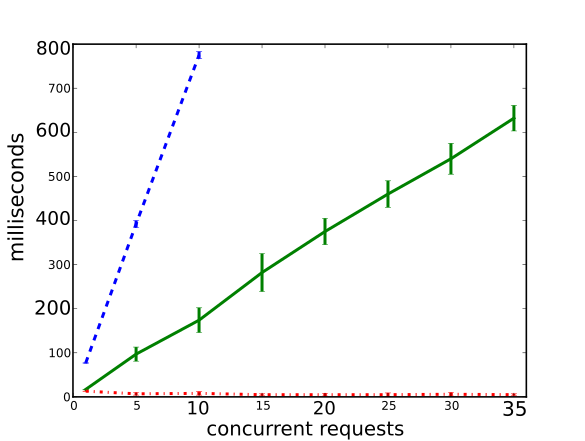
\includegraphics[width=3in]{images/device_comparison.png}
% \label{fig:deviceCompatison}
% \caption{Time measurement comparison among XBee sensors, FoxG20 and a regular computer}
% \end{figure}




\InsertFig{device_comparison}{fig:deviceComparison}{
  Response times measured in different embedded devices
}{
  The dash-dotted line represents the regular computer, the solid line the FoxG20 and the dashed line the XBee.
}{0.7}{}


\begin{table}[htbp]
    \caption{Mean of the measurements taken in different devices with the standard deviation ($\sigma$) in parenthesis.}
    \centering
    \begin{tabular}{|c|c|c|c|}
      \hline
      Concurrent & XBee & FoxG20 & Regular \\
      requests   &  & &  computer \\
      \hline
      1  &  77 (1)	&  17 (0)  &  13 (0) \\
      5  & 392 (8)	&  97 (16) &   7 (3) \\
      10 & 775 (8)	& 174 (28) &   8 (4) \\
      15 &  -	& 282 (43) &   5 (2) \\
      20 &  -	& 375 (30) &   5 (3) \\
      25 &  -	& 460 (30) &   5 (4) \\
      30 &  -	& 540 (35) &   6 (4) \\
      35 &  -	& 632 (29) &   5 (2) \\
      \hline
    \end{tabular}
    \label{tab:timeMeasures}
\end{table}
\section{Conclusion}
% 2. Comparativa
\label{sec:tsc_wot_conclusion}

% 5. otra forma de aunar las ventajas de ambos? => construir un TSC compatible con WoT (on top of that) <= integración profunda
%	Ventajas:
%		+ interoperable with other semantic WoT systems
%		+ syntactic services can still be provided using a different type of representation => WoT
%		+ promote indirect communication style => abstraction for the developer (does not care about manually discovering interfaces)
%	Problemas:
%		+ necesitas out-of-the-band conocimiento? API fija?
% esto trae problemas: cap 4 y cap 5


This chapter compares two different resource oriented approaches for the \acl{iot}: \acl{wot} and \acl{tsc}.
\ac{wot} seems to scale in a better way thanks to the underlying HTTP protocol, while \ac{tsc} performs the discovery process among locally available network-connected objects in a seamless way.
The first one is more human oriented and the second one relies on the Semantic Web capabilities to exchange a machine processable data.
Furthermore, the second one is ideal to easily configure intranets of network connected objects whilst the first one can easily bridge those intranets configuring global multi-site IoT ecosystems.

We deem that both approaches can win much from their combination since the weaknesses of one are outweighed by the strengths of the other.
Hence, they can be combined to offer a more scalable, machine and human processable solution that offers better cooperation possibilities among internet-connected objects and thus aid users in their daily activities.
As a simple proof of this hypothesis, a scenario employing \ac{wot} to export each space data to the outer world and \ac{tsc} to enable seamless and automatic configuration of heterogeneous devices on local networks has been presented.